\section{Force approximation error and performance}
The ``local picture'' of the errors of force approximation in the \PThreeM{} method has already been outlined in \autoref{fig:reference-force-combined}.
Now we turn to investigate how the choice of the particle shape ($S_1$ or $S_2$) and the size of the particle diameter influences the global force approximation error.
The error is defined exactly the same as in the case of the PM method, i.e. we use \autoref{eq:force-avg-relative-err}.

In our test, the grid covering the computational region had dimensions of $64\times 64\times 32$ and $N=10{,}000$ particles were used.
The result of the test is shown in \autoref{fig:p3m-global-err}.
\begin{figure}[htp]
    \centering
    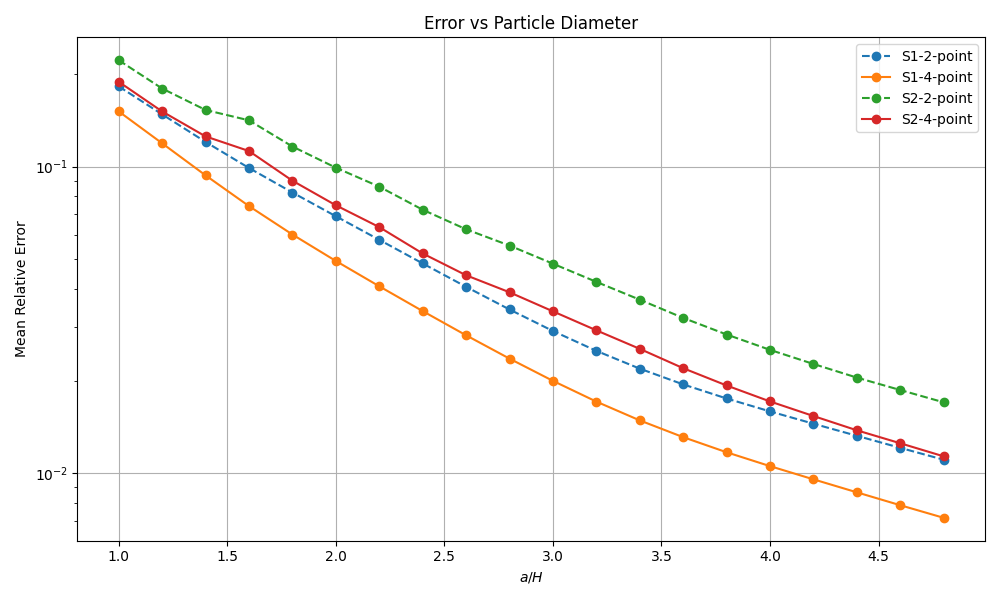
\includegraphics[scale=0.5]{img/err_vs_part_diam_p3m.png}
    \caption{Mean relative error in P3M approximation.}
    \label{fig:p3m-global-err}
\end{figure}
The figure clearly illustrates that the error drops with increasing the size of the particle diameter $a$.
This is an expected result, since with increasing $a$, the P3M method calculates more interparticle forces through exact direct summation.
Moreover, as we could see in \autoref{fig:reference-force-error-sub}, the PM approximation to the reference force gets better with increasing particle diameter.
These two effects combined are responsible for the reduction of the global error.

For both the $S_1$ and $S_2$ shapes, the error was minimized when the fourth-order finite difference was used for gradient calculation, as one could obviously expect.
The test indicated superiority of the $S_1$ shape, with the difference between the two becoming more significant for bigger relative values of $a$.